% Chapter Template

\chapter{Future Work} % Main chapter title

\label{Chapter8} % Change X to a consecutive number; for referencing this chapter elsewhere, use \ref{ChapterX}

\lhead{Chapter 8. \emph{Future Work}} % Change X to a consecutive number; this is for the header on each page - perhaps a shortened title

%----------------------------------------------------------------------------------------
%	SECTION 1
%----------------------------------------------------------------------------------------

\section{What Comes Next?}
The experiments layed out in the previous chapters have shown that MRL using MAEs allows for the unsupervised learning of a grounded representation of images and language. How then, can this be used to improve robotic technologies?

I see many potential applications for MRl within the field of Human Robot Interaction (HRI). \autoref{fig:fsm} shows an example of how the MAE can be included ina robotic system.


\begin{figure}
\centering
\includegraphics[width=\textwidth]{Figs/futureWork/fsm.png}
\caption{An example of how the MAE can be used as part of a robotic system.}
\label{fig:fsm}
\end{figure}

Consider the scenario of a human interacting with a robot to teach it a set of objects and their visual attributes as well as the words used to describe the objects and their visual attributes. In a laboratory setting it is feasable to have only a single object in view at any given time. This is not true for real world scenarios. However, with the introduction of a simple finite state machine (FSM) controlled via a Natural Language Understanding (NLU) module, it is simple to use an MAE trained with MRL to discern which object is being referred to by the human. This is demonstrated in \autoref{fig:disamb}

\begin{figure}
\centering
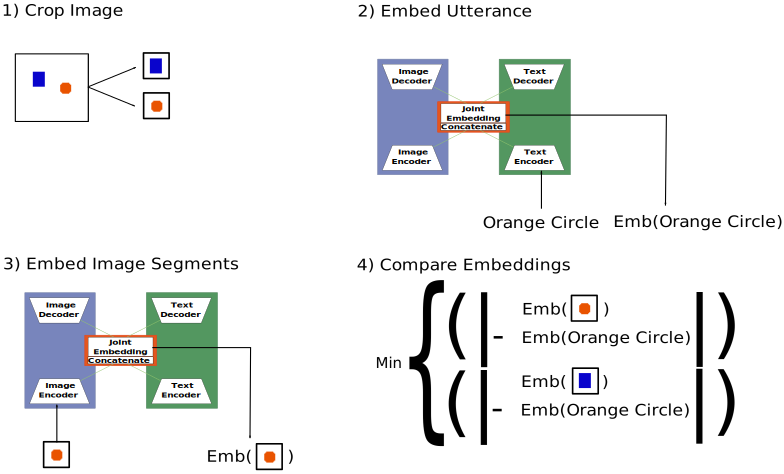
\includegraphics[width=\textwidth]{Figs/shapes/findingRefferant.png}
\caption{An example of using an MAE trained with MRL to disambiguate which object is being referred to in a scene.}
\label{fig:disamb}
\end{figure}

In order for the scenario depicted in \ref{fig:disamb}, an NLU module must be trained to extract the Intent of the human's utterance as well as any Entities which the human refers to. Fortunately, these types of NLUs are easily built using open source libraries like Rasa \cite{rasa}.




%-----------------------------------
%	SUBSECTION 1
%-----------------------------------
